\documentclass[sigconf,authorversion]{acmart}
\usepackage[utf8]{inputenc}
\usepackage{booktabs}
\usepackage{enumitem} %resume enumerate
\usepackage{graphicx}
\usepackage{caption}
\usepackage{subcaption}

% Remove reference format
\settopmatter{printacmref=false}
\setcopyright{none}
\renewcommand\footnotetextcopyrightpermission[1]{}
\pagestyle{plain}

\title{SGEMM Product Analysis}
\author{Roger Pujol}
\affiliation{%
  \institution{Universitat Politècnica de Catalunya (UPC)}
  \city{Barcelona}
  \country{Spain}}
% \affiliation{%
%   \institution{Barcelona Supercomputing Center (BSC)}
%   \city{Barcelona}
%   \country{Spain}}
\email{roger.pujol.torramorell@est.fib.upc.edu}
\date{\today}

\begin{abstract}
General Matrix Multiplications (GEMM) are a key component in the rising world of Deep Learning. Most of the computational complexity of Deep Neural Networks can be reduced to mutliple huge GEMMs. Since any small optimization in GEMM can affect positively in many applications, our objective in this project will be to find how the parameters affect the performance of this kind of operations. Also we will try to get a regressor model capable to predict the time that will be needed to compute the GEMM given the parameters used.\\
The code of this project is Open Source and can be found in: \url{https://github.com/rogerpt32/adm_paper1}
\end{abstract}

\begin{document}

\maketitle

\section{Introduction}
\section{Data set}
The dataset used is from the UCI Machine Learning Repository \cite{dataset-url} \cite{dataset-paper}. This data set measures the running time of a matrix-matrix product A*B = C, where all matrices have size 2048 x 2048, using a parameterizable SGEMM (the ``S'' stands for ``Single precision'', meaning 32 bits floating point) GPU kernel with 241600 possible parameter combinations. For each tested combination, 4 runs were performed and their results are reported as the 4 last columns. All times are measured in milliseconds*. \\
There are 14 parameter, the first 10 are ordinal and can only take up to 4 different powers of two values, and the 4 last variables are binary. Out of 1327104 total parameter combinations, only 241600 are feasible (due to various kernel constraints). This data set contains the results for all these feasible combinations.\\
The values of the data set were taken using a desktop workstation running Ubuntu 16.04 Linux with an Intel Core i5 (3.5GHz), 16GB RAM, and a NVidia Geforce GTX 680 4GB GF580 GTX-1.5GB GPU. The tool used was the ``gemm\_fast'' kernel from the automatic OpenCL kernel tuning library ``CLTune''.
\subsection{Attribute information}
\textbf{Independent variables:}
\begin{enumerate}
  \item  MWG: per-matrix 2D tiling at workgroup level: {16, 32, 64, 128} (integer)
  \item NWG: per-matrix 2D tiling at workgroup level: {16, 32, 64, 128} (integer)
  \item KWG: inner dimension of 2D tiling at workgroup level: {16, 32} (integer)
  \item MDIMC: local workgroup size: {8, 16, 32} (integer)
  \item NDIMC: local workgroup size: {8, 16, 32} (integer)
  \item MDIMA: local memory shape: {8, 16, 32} (integer)
  \item NDIMB: local memory shape: {8, 16, 32} (integer)
  \item KWI: kernel loop unrolling factor: {2, 8} (integer)
  \item VWM: per-matrix vector widths for loading and storing: {1, 2, 4, 8} (integer)
  \item VWN: per-matrix vector widths for loading and storing: {1, 2, 4, 8} (integer)
  \item STRM: enable stride for accessing off-chip memory within a single thread: {0, 1} (categorical)
  \item STRN: enable stride for accessing off-chip memory within a single thread: {0, 1} (categorical)
  \item SA: per-matrix manual caching of the 2D workgroup tile: {0, 1} (categorical)
  \item SB: per-matrix manual caching of the 2D workgroup tile: {0, 1} (categorical)
\end{enumerate}

\textbf{Output:}
\begin{enumerate}[resume]
  \item Run1: performance times in milliseconds for an independent run using the parameters described in the previous attributes.
  \item Run2: another independent run (see Run1).
  \item Run3: another independent run (see Run1).
  \item Run4: another independent run (see Run1).
\end{enumerate}
The range of the running times is between 13.25 and 3397.08.
\section{Preprocess}
Since this dataset is very synthetic because of its computational nature, there isn't much things to preprocess. The only thing that we have done to preprocess the data, has been to separate each Run in a unique row, which only has one Run. This means that after the pre process we have 3 less columns but 4 times more rows. This new dataset have a lot of redundand data compared to the original version but is easier to handle, since now there is only one target variable.
\section{Analysis}
In this section we will do a very brief analysis of the impact of the variables to the target variable (Run). To do this analysis, we have plots with all the dataset points where the Y-axis is always the target variable and then in each plot the X-axis is a different variable.\\
With this we can see that MWG \ref{fig:mwg} and NWG \ref{fig:nwg} have a big impact where a smaller values will always have small results but bigger values have a bigger variance in the results. This same effect can be seen but less clearly in KWG \ref{fig:kwg}, KWI \ref{fig:kwi}, SA \ref{fig:sa} and SB \ref{fig:sb}, which could mean that this variables are a bit less important and depend more on other variables. Then in MDIMC \ref{fig:mdimc} and NDIMC \ref{fig:ndimc} have the opposite impact to MWG and NWG, here the bigger values implies small results but smaller values have bigger variance in the results.\\
Finally the other variables (MDIMA \ref{fig:mdima}, NDIMB \ref{fig:ndimb}, VWM \ref{fig:vwm}, VWN \ref{fig:vwn}, STRM \ref{fig:strm} and STRN \ref{fig:strn}) doesn't seem to have a direct implication since for any value have a similar distribution in the target. This doesn't mean that this variables are useless, this means that their value alone doesn't clarify anithing about the target but it might be meaningful only when combined with other variables.
\begin{figure*}[htb]
    \centering
    \begin{subfigure}[b]{0.3\textwidth}
        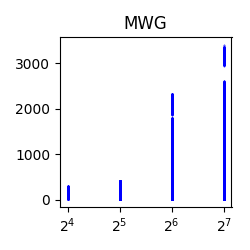
\includegraphics[width=\textwidth]{img/MWG.png}
        \subcaption{MWG}
        \label{fig:mwg}
    \end{subfigure}
%
    \begin{subfigure}[b]{0.3\textwidth}
        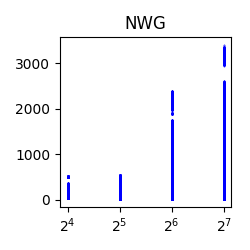
\includegraphics[width=\textwidth]{img/NWG.png}
        \subcaption{NWG}
        \label{fig:nwg}
    \end{subfigure}
    % \caption{$Q^{*}$ values for different arms}
    \begin{subfigure}[b]{0.3\textwidth}
        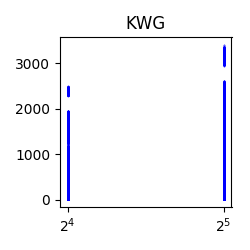
\includegraphics[width=\textwidth]{img/KWG.png}
        \subcaption{KWG}
        \label{fig:kwg}
    \end{subfigure}
\end{figure*}
\begin{figure*}[htb]\ContinuedFloat
    \centering
    \begin{subfigure}[b]{0.3\textwidth}
        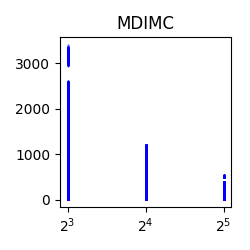
\includegraphics[width=\textwidth]{img/MDIMC.png}
        \subcaption{MDIMC}
        \label{fig:mdimc}
    \end{subfigure}
    \begin{subfigure}[b]{0.3\textwidth}
        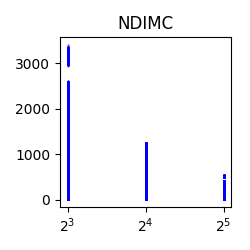
\includegraphics[width=\textwidth]{img/NDIMC.png}
        \subcaption{MDIMC}
        \label{fig:ndimc}
    \end{subfigure}
    \begin{subfigure}[b]{0.3\textwidth}
        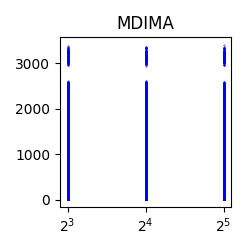
\includegraphics[width=\textwidth]{img/MDIMA.png}
        \subcaption{MDIMA}
        \label{fig:mdima}
    \end{subfigure}
\end{figure*}
\begin{figure*}[htb]\ContinuedFloat
    \centering
    \begin{subfigure}[b]{0.3\textwidth}
        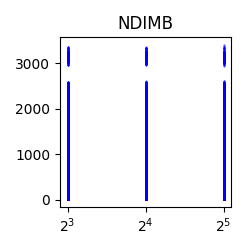
\includegraphics[width=\textwidth]{img/NDIMB.png}
        \subcaption{NDIMB}
        \label{fig:ndimb}
    \end{subfigure}
    \begin{subfigure}[b]{0.3\textwidth}
        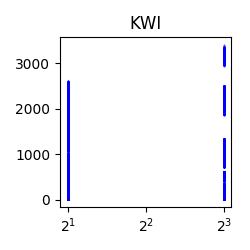
\includegraphics[width=\textwidth]{img/KWI.png}
        \subcaption{KWI}
        \label{fig:kwi}
    \end{subfigure}
    \begin{subfigure}[b]{0.3\textwidth}
        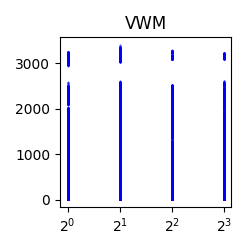
\includegraphics[width=\textwidth]{img/VWM.png}
        \subcaption{VWM}
        \label{fig:vwm}
    \end{subfigure}
\end{figure*}
\begin{figure*}[htb]\ContinuedFloat
    \centering
    \begin{subfigure}[b]{0.3\textwidth}
        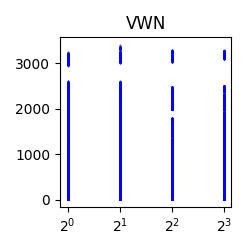
\includegraphics[width=\textwidth]{img/VWN.png}
        \subcaption{VWN}
        \label{fig:vwn}
    \end{subfigure}
    \begin{subfigure}[b]{0.3\textwidth}
        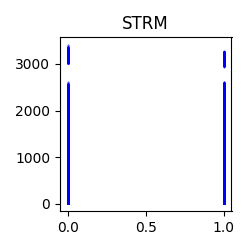
\includegraphics[width=\textwidth]{img/STRM.png}
        \subcaption{STRM}
        \label{fig:strm}
    \end{subfigure}
    \begin{subfigure}[b]{0.3\textwidth}
        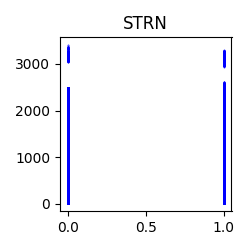
\includegraphics[width=\textwidth]{img/STRN.png}
        \subcaption{STRN}
        \label{fig:strn}
    \end{subfigure}
\end{figure*}
\begin{figure*}[htb]\ContinuedFloat
    \centering
    \begin{subfigure}[b]{0.3\textwidth}
        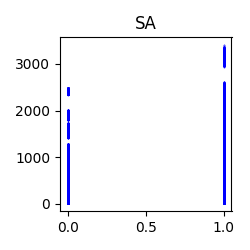
\includegraphics[width=\textwidth]{img/SA.png}
        \subcaption{SA}
        \label{fig:sa}
    \end{subfigure}
    \begin{subfigure}[b]{0.3\textwidth}
        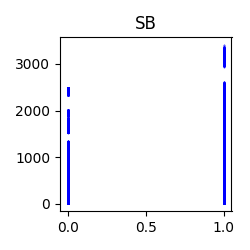
\includegraphics[width=\textwidth]{img/SB.png}
        \subcaption{SB}
        \label{fig:sb}
    \end{subfigure}
    \caption{Plots of all variables contrasted with the target variable. Note that in most of the plots the X-axis is logarithmic.}
    \label{fig:plots}
\end{figure*}
\section{Regression Line Model}
The first approach that we used to try to predict the execution time of the SGEMM given the parameters, is a simple regression line.
\subsection{Implementation}
To get the model, first we split the model in two blocks: one for training (in this case 90\% of the data set) and the other to test (in this case 10\% of the data set) the accuracy later. Then we use the training part to fit the regression line model. Finally we use that model to predict the execution times of the test examples and we compare the results with the real values.
\subsection{Results}
The results from the Regression Line are not very satisfying. The mean square error that this model has in the training data is 80322.28, and obviously the mean square error in the testing data is even worse with a value of 82841.39. This lack of accuracy using a linear regression, might probably mean that our data is not linear. If we check the variance using the $R^2$-score, where a 1 means that the data fits perfectly to the regression line with no variance and a 0 means the opposite, we get a 0.41 in both train and test data. This confirms that this regression might not be a good solution.\\
But in order to benefit from this model, we can take a look to the coefficients that define the model. This coefficients multiply the correspondent input variables described in the Data Set section.
\begin{itemize}
  \item 3.3280371
  \item 3.07243576
  \item 5.1729495
  \item -16.67627391
  \item -16.33800475
  \item 1.01720931
  \item 1.02988438
  \item 3.98709287
  \item -1.52596645
  \item -3.01457498
  \item -9.44404773
  \item -0.18646408
  \item 37.88273766
  \item 46.99629411
\end{itemize}
With this we can see that as we predicted in the analysis of the data: MWG, NWG, KWG, KWI, SA and SB have a positive impact in the target (bigger input means bigger execution time), whereas MDIMC and NDIMC have a negative impact in the target (bigger input means smaller execution time).
\section{Decision Tree Regressor Model}
The second approach to fit the data to a model is using decision trees.
\subsection{Implementation}
The implementation of this method has followed a similar steps to the Regression Line Model. First we split the data in training (75\%) and test (25\%). Then with the training data we fitted two decision tree models, one without any restrictions and another with the depth limited to 5. After that we test the accuracy of both models with training and test data (separately).
\subsection{Results}
\begin{table}[htbp]
\begin{tabular}{lcc}
  \toprule
  & Full DT model & DT max depth 5 \\
  \midrule
  Max Depth & 25 & 5 \\
  Node Count & 481085 & 63 \\
  MSE train & 3.55 & 31092.63 \\
  $R^2$ train & 1 & 0.77 \\
  MSE test & 8.39 & 30345.53 \\
  $R^2$ test & 1 & 0.77 \\
  \bottomrule
\end{tabular}
\caption{Results from the decision tree models}
\label{tab:dt}
\end{table}
The model trained without restrictions have a great accuracy since the mean square error in training is only 3.55 and in test is 8.39. But this impressive accuracy is basically consequence of a huge overfitting. If we check the depth and the number of nodes of the model (see table \ref{tab:dt}), we can see that basically the model has probably almost one leaf for each possible configuration. Technically since we have all the possible configurations encoded in this decision tree, the results will be always accurate, but if we want to extract useful information from this model it will be very hard.\\
To analyse easily the impact of the variables we use the model trained with the maximum depth fixed to 5. This restriction reduce the depth from the previous model to 5 and the node count to only 63. Taking a look to the values of each decision node (see the file \textit{doc/tree/tree.pdf} from the githb repository given in the abstract) we can see that only a few variables are used. The variables used are: MWG, NWG, MDIMC, NDIMC and SA. These confirm again what we saw at the analysis of the data where the mentioned variables were the ones with more importance on the final result. The accuracy of this reduced model is worse than the full one (see table \ref{tab:dt}), which is obvious since we are only using 5 variables and not checking all the configurations, but still it has a better accuracy than the simple regression line.
\section{Conclusions}

\bibliographystyle{unsrt}
\bibliography{cites}

\end{document}
